%----------------------------------------------------------
\chapter{Тестирование и отладка}\label{chap4_soft_testing}
%----------------------------------------------------------

Реализованный алгоритм поиска циклов в графе позволяет находить все циклы в загружаемой или создаваемой графовой модели и выполнять их подсветку. В качестве примеров рассмотрим несколько графовых моделей: на рисунке (\ref{fig:example_no_cycles}) приведен граф, который не содержит ни одного цикла, соответственно после выполнения поиска циклов не будет найдено ни одного цикла, поэтому ни вершины ни ребра подсвечены не будут.

\begin{figure}[ht!]
\center{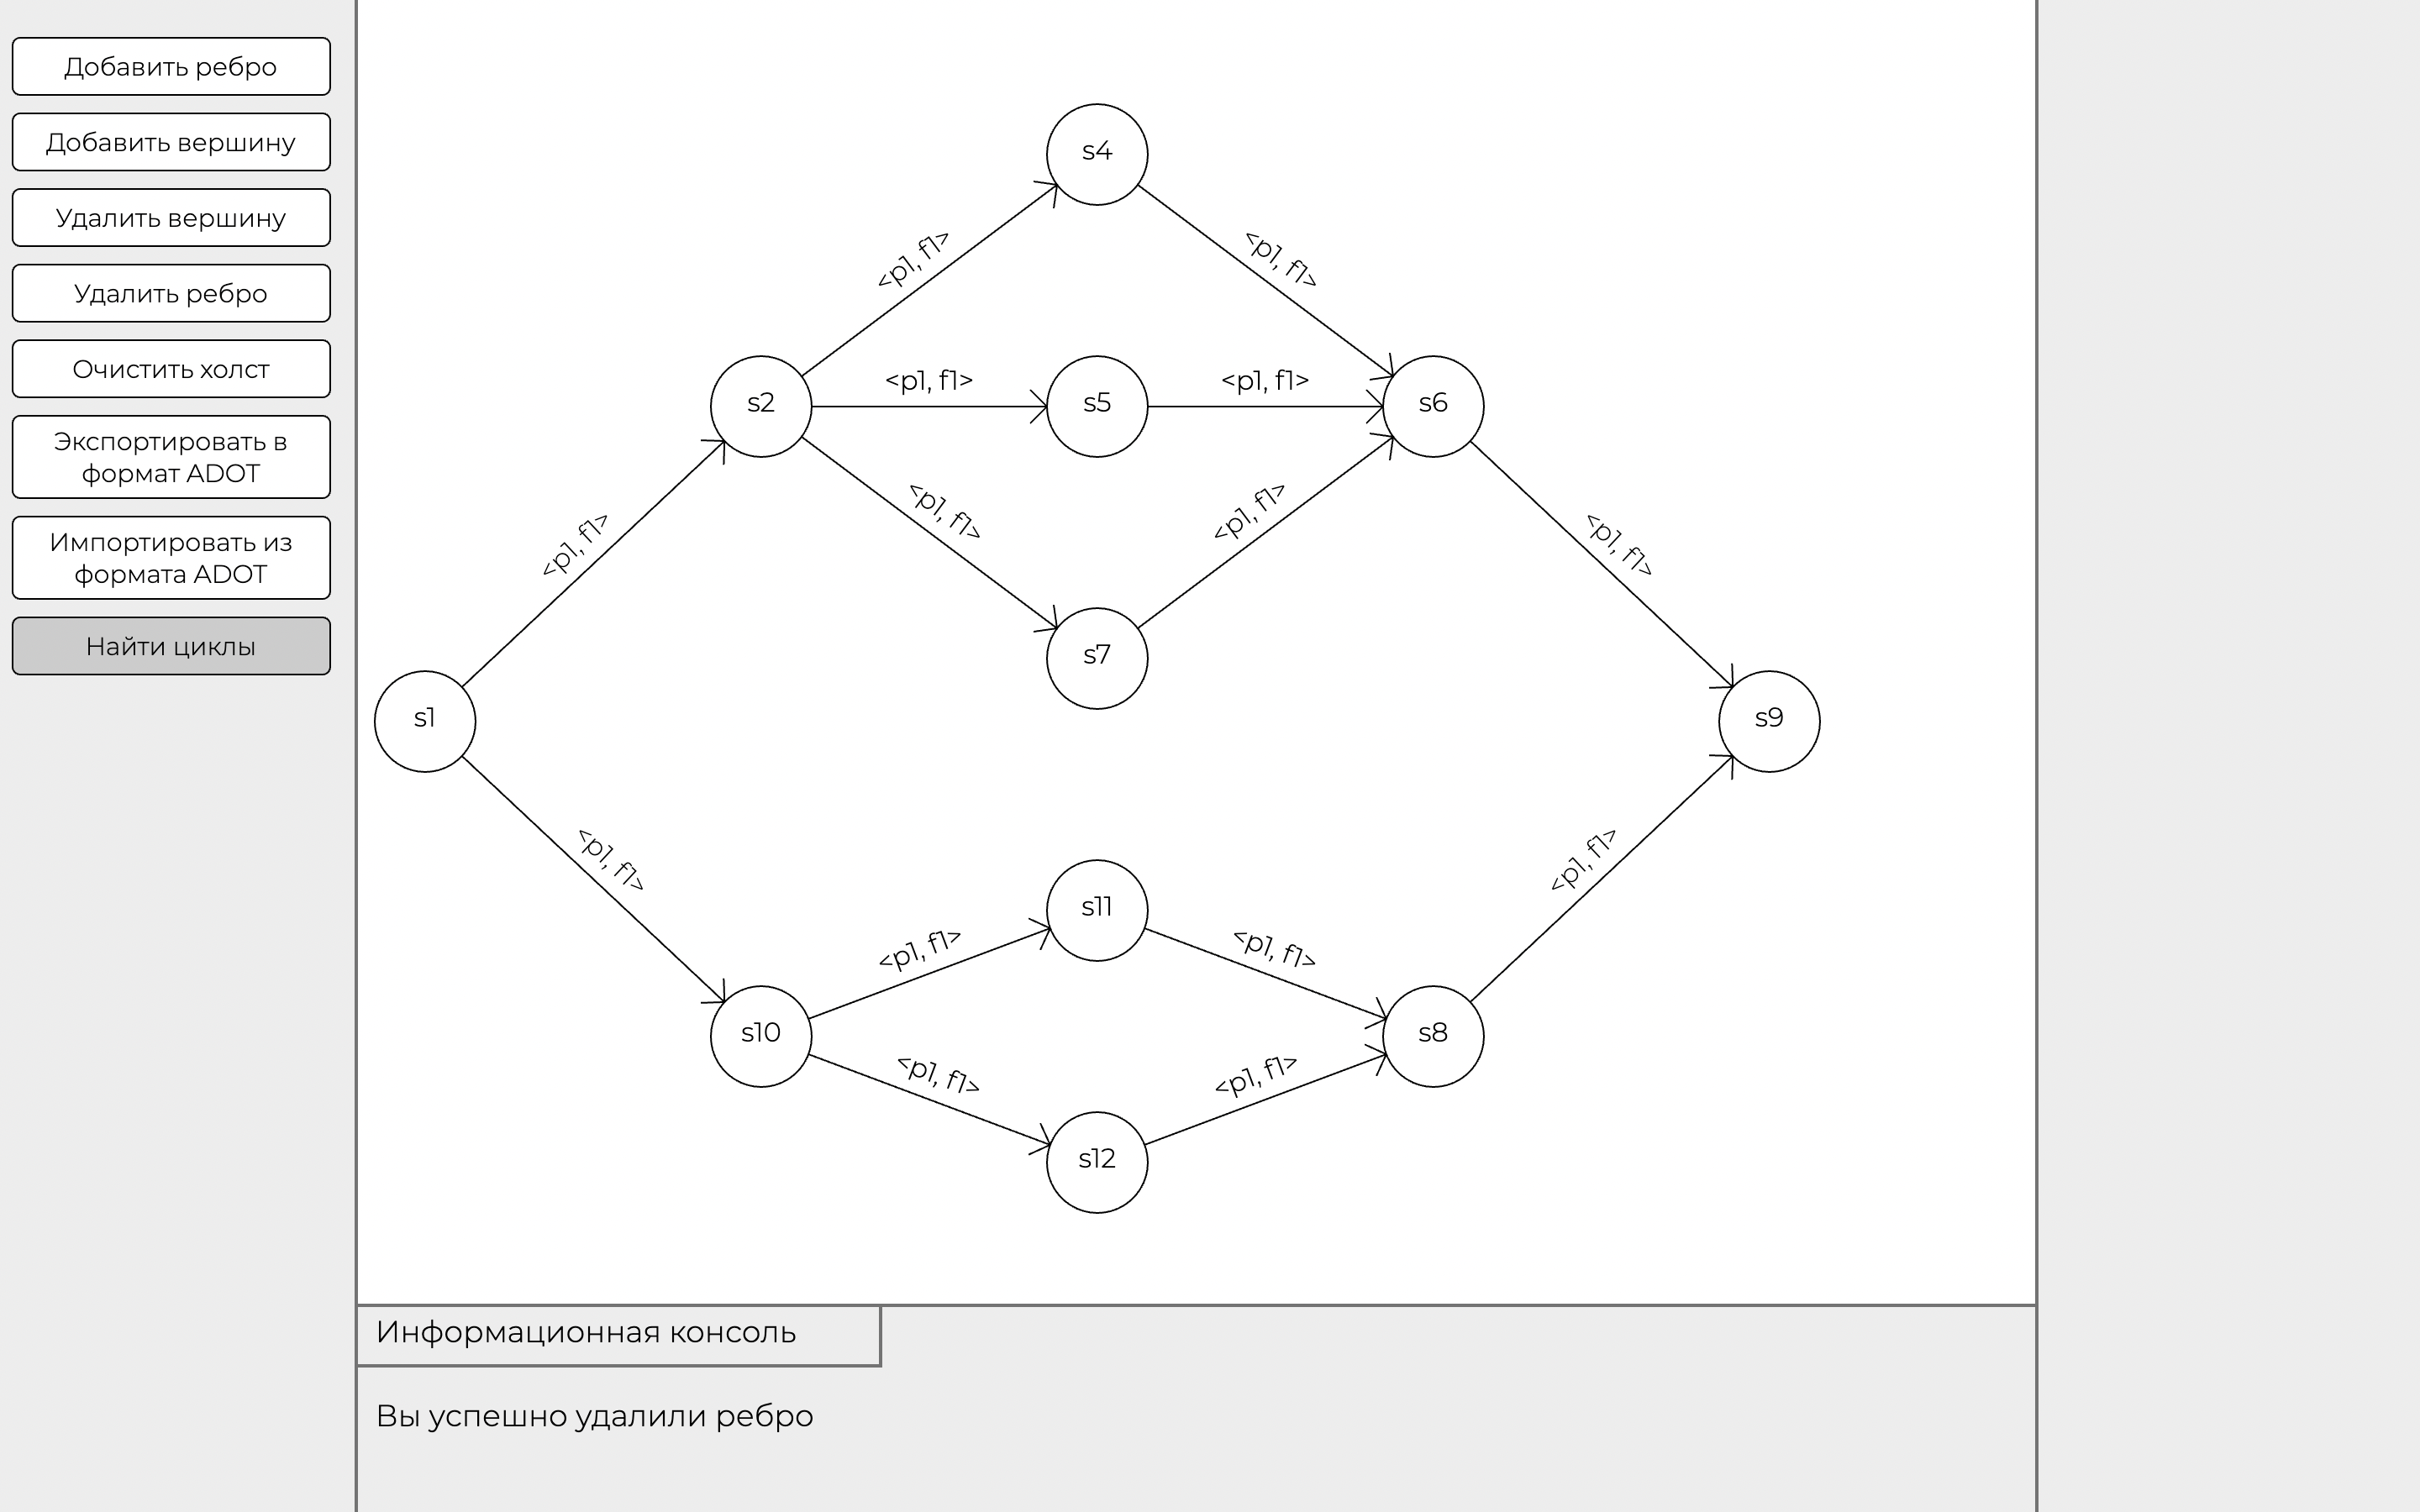
\includegraphics[width=0.75\linewidth]{images/example_no_cycles.png}}
\caption{Граф без циклов}
\label{fig:example_no_cycles}
\end{figure}

На рисунке (\ref{fig:example_one_cycle}) в графе присутствует только один цикл, после выполнения поиска циклов данный цикл будет найден и подсвечен.

\begin{figure}[ht!]
\center{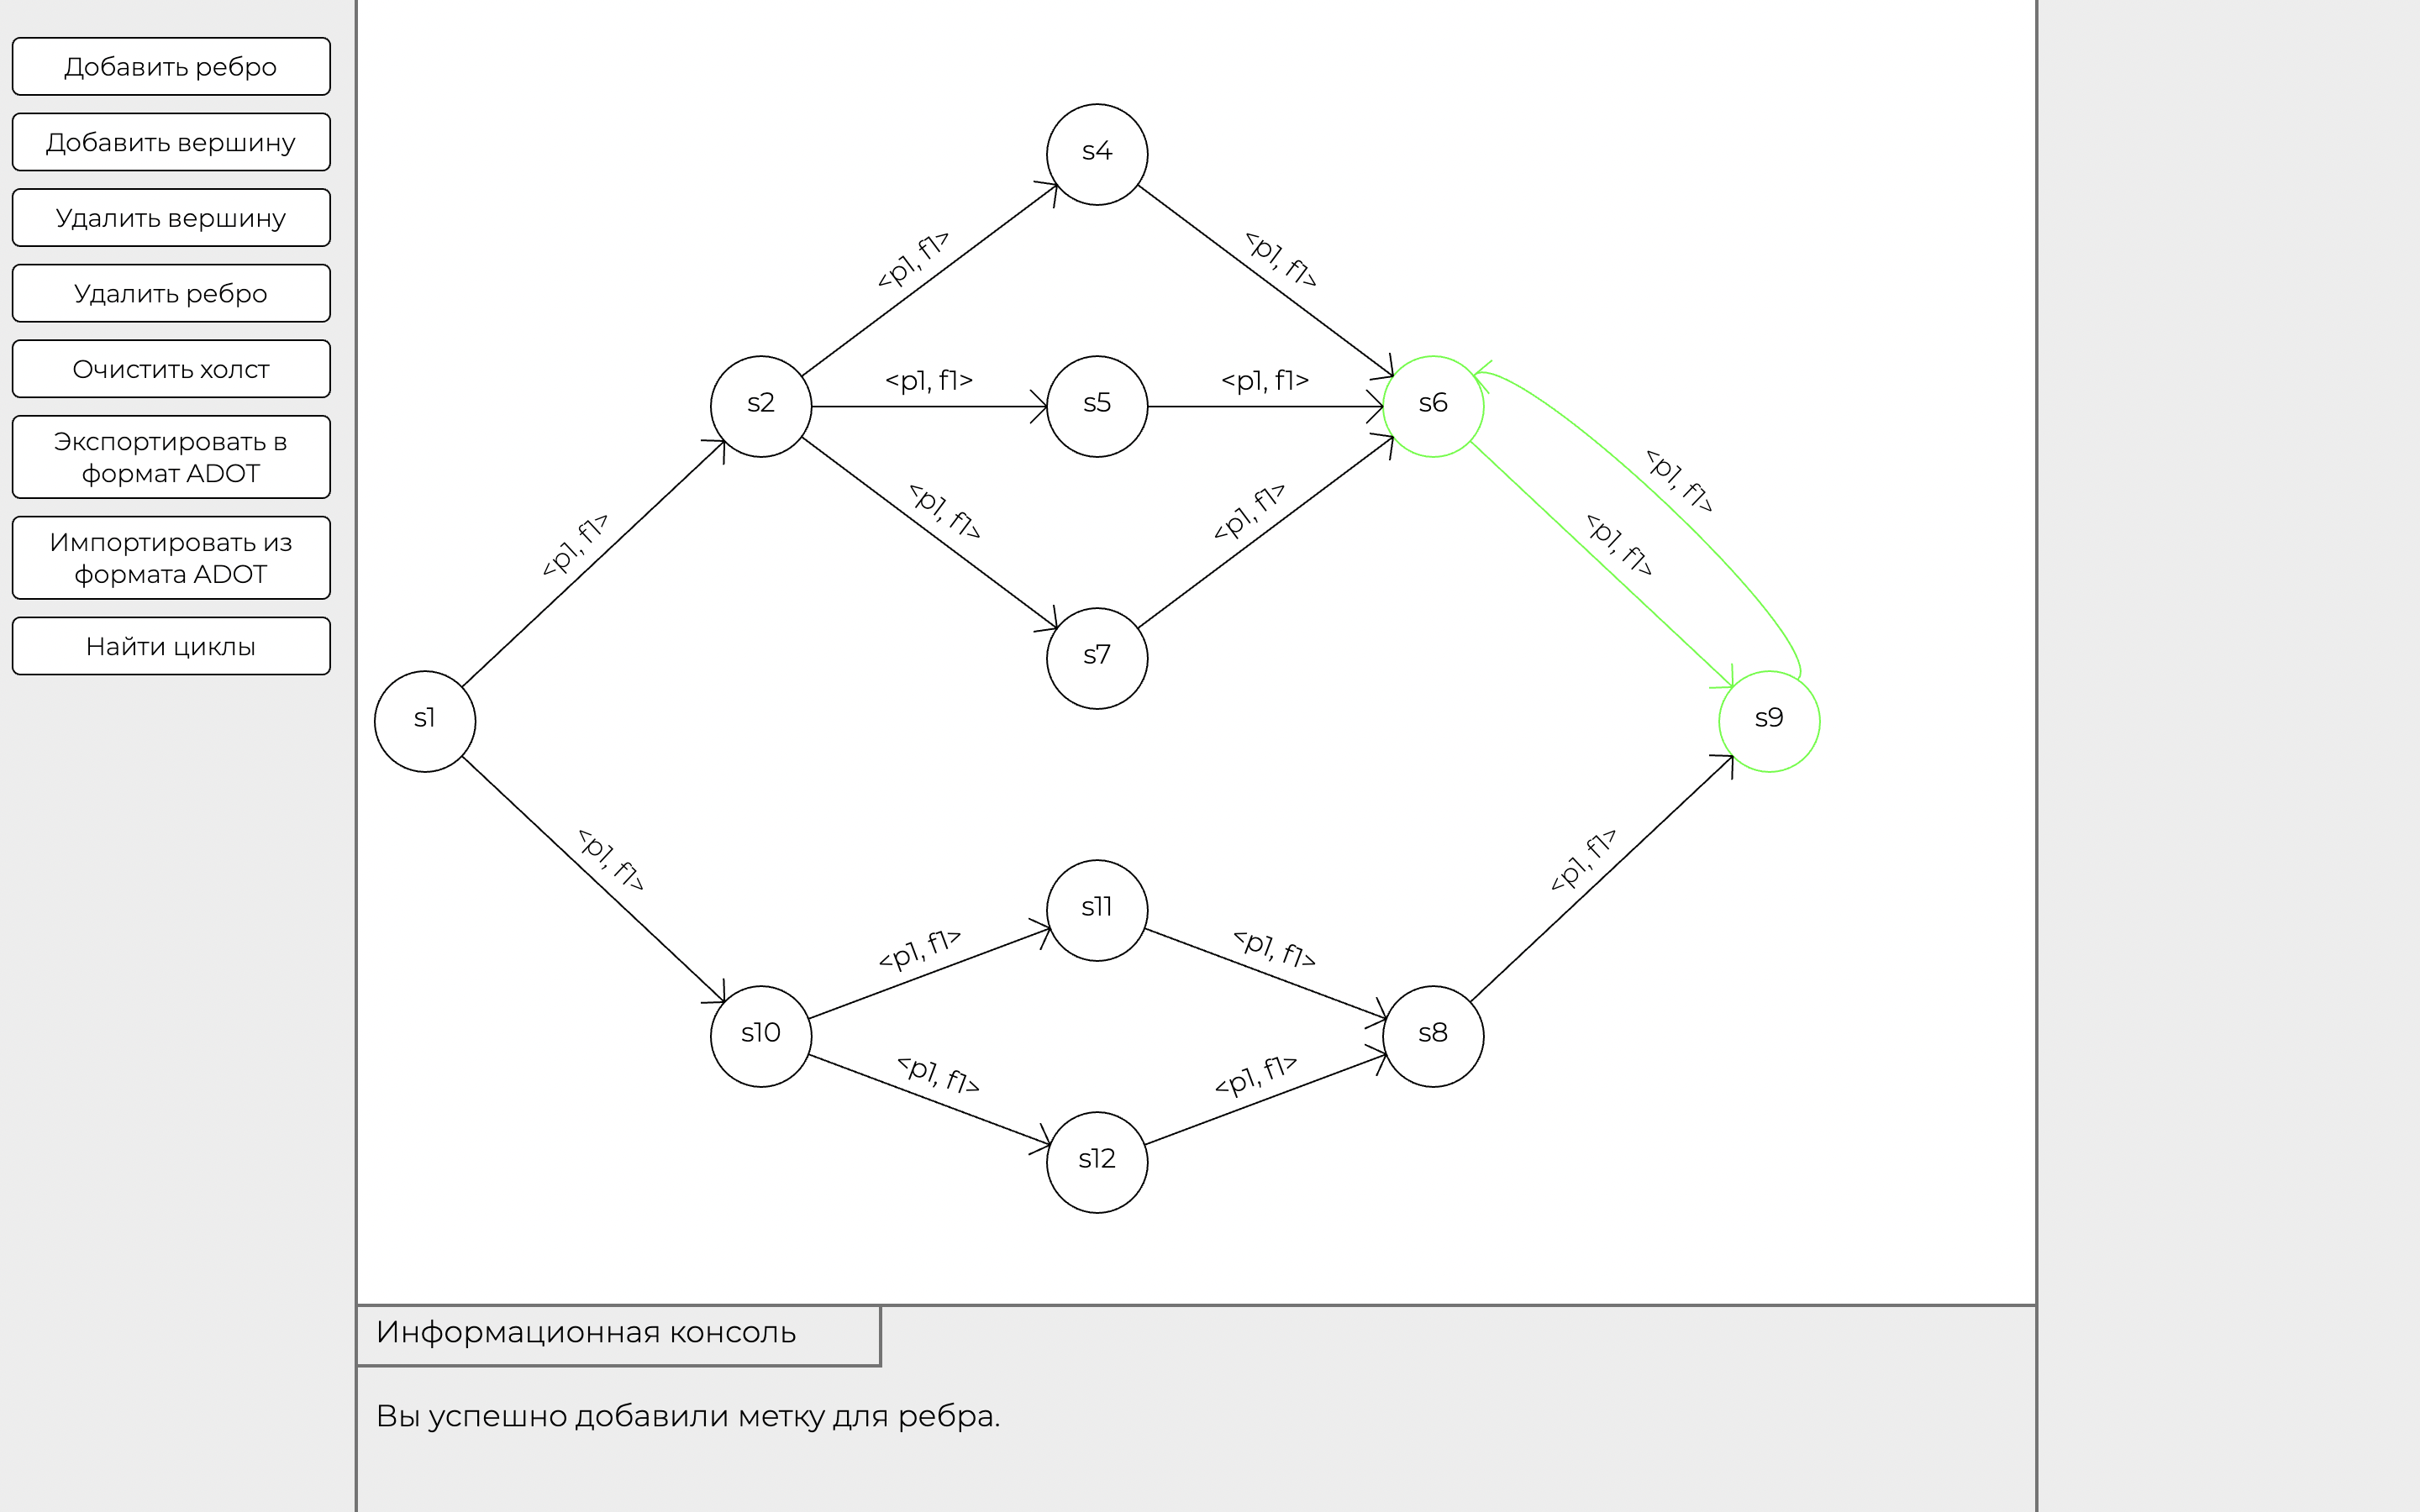
\includegraphics[width=0.75\linewidth]{images/example_one_cycle.png}}
\caption{Граф c одним простым циклом}
\label{fig:example_one_cycle}
\end{figure}

В приведенном на рисунке (\ref{fig:example_many_cycles}) графе присутствует множество циклов, в результате поиска циклов абсолютно все циклы были найдены и подсвечены.

\begin{figure}[ht!]
\center{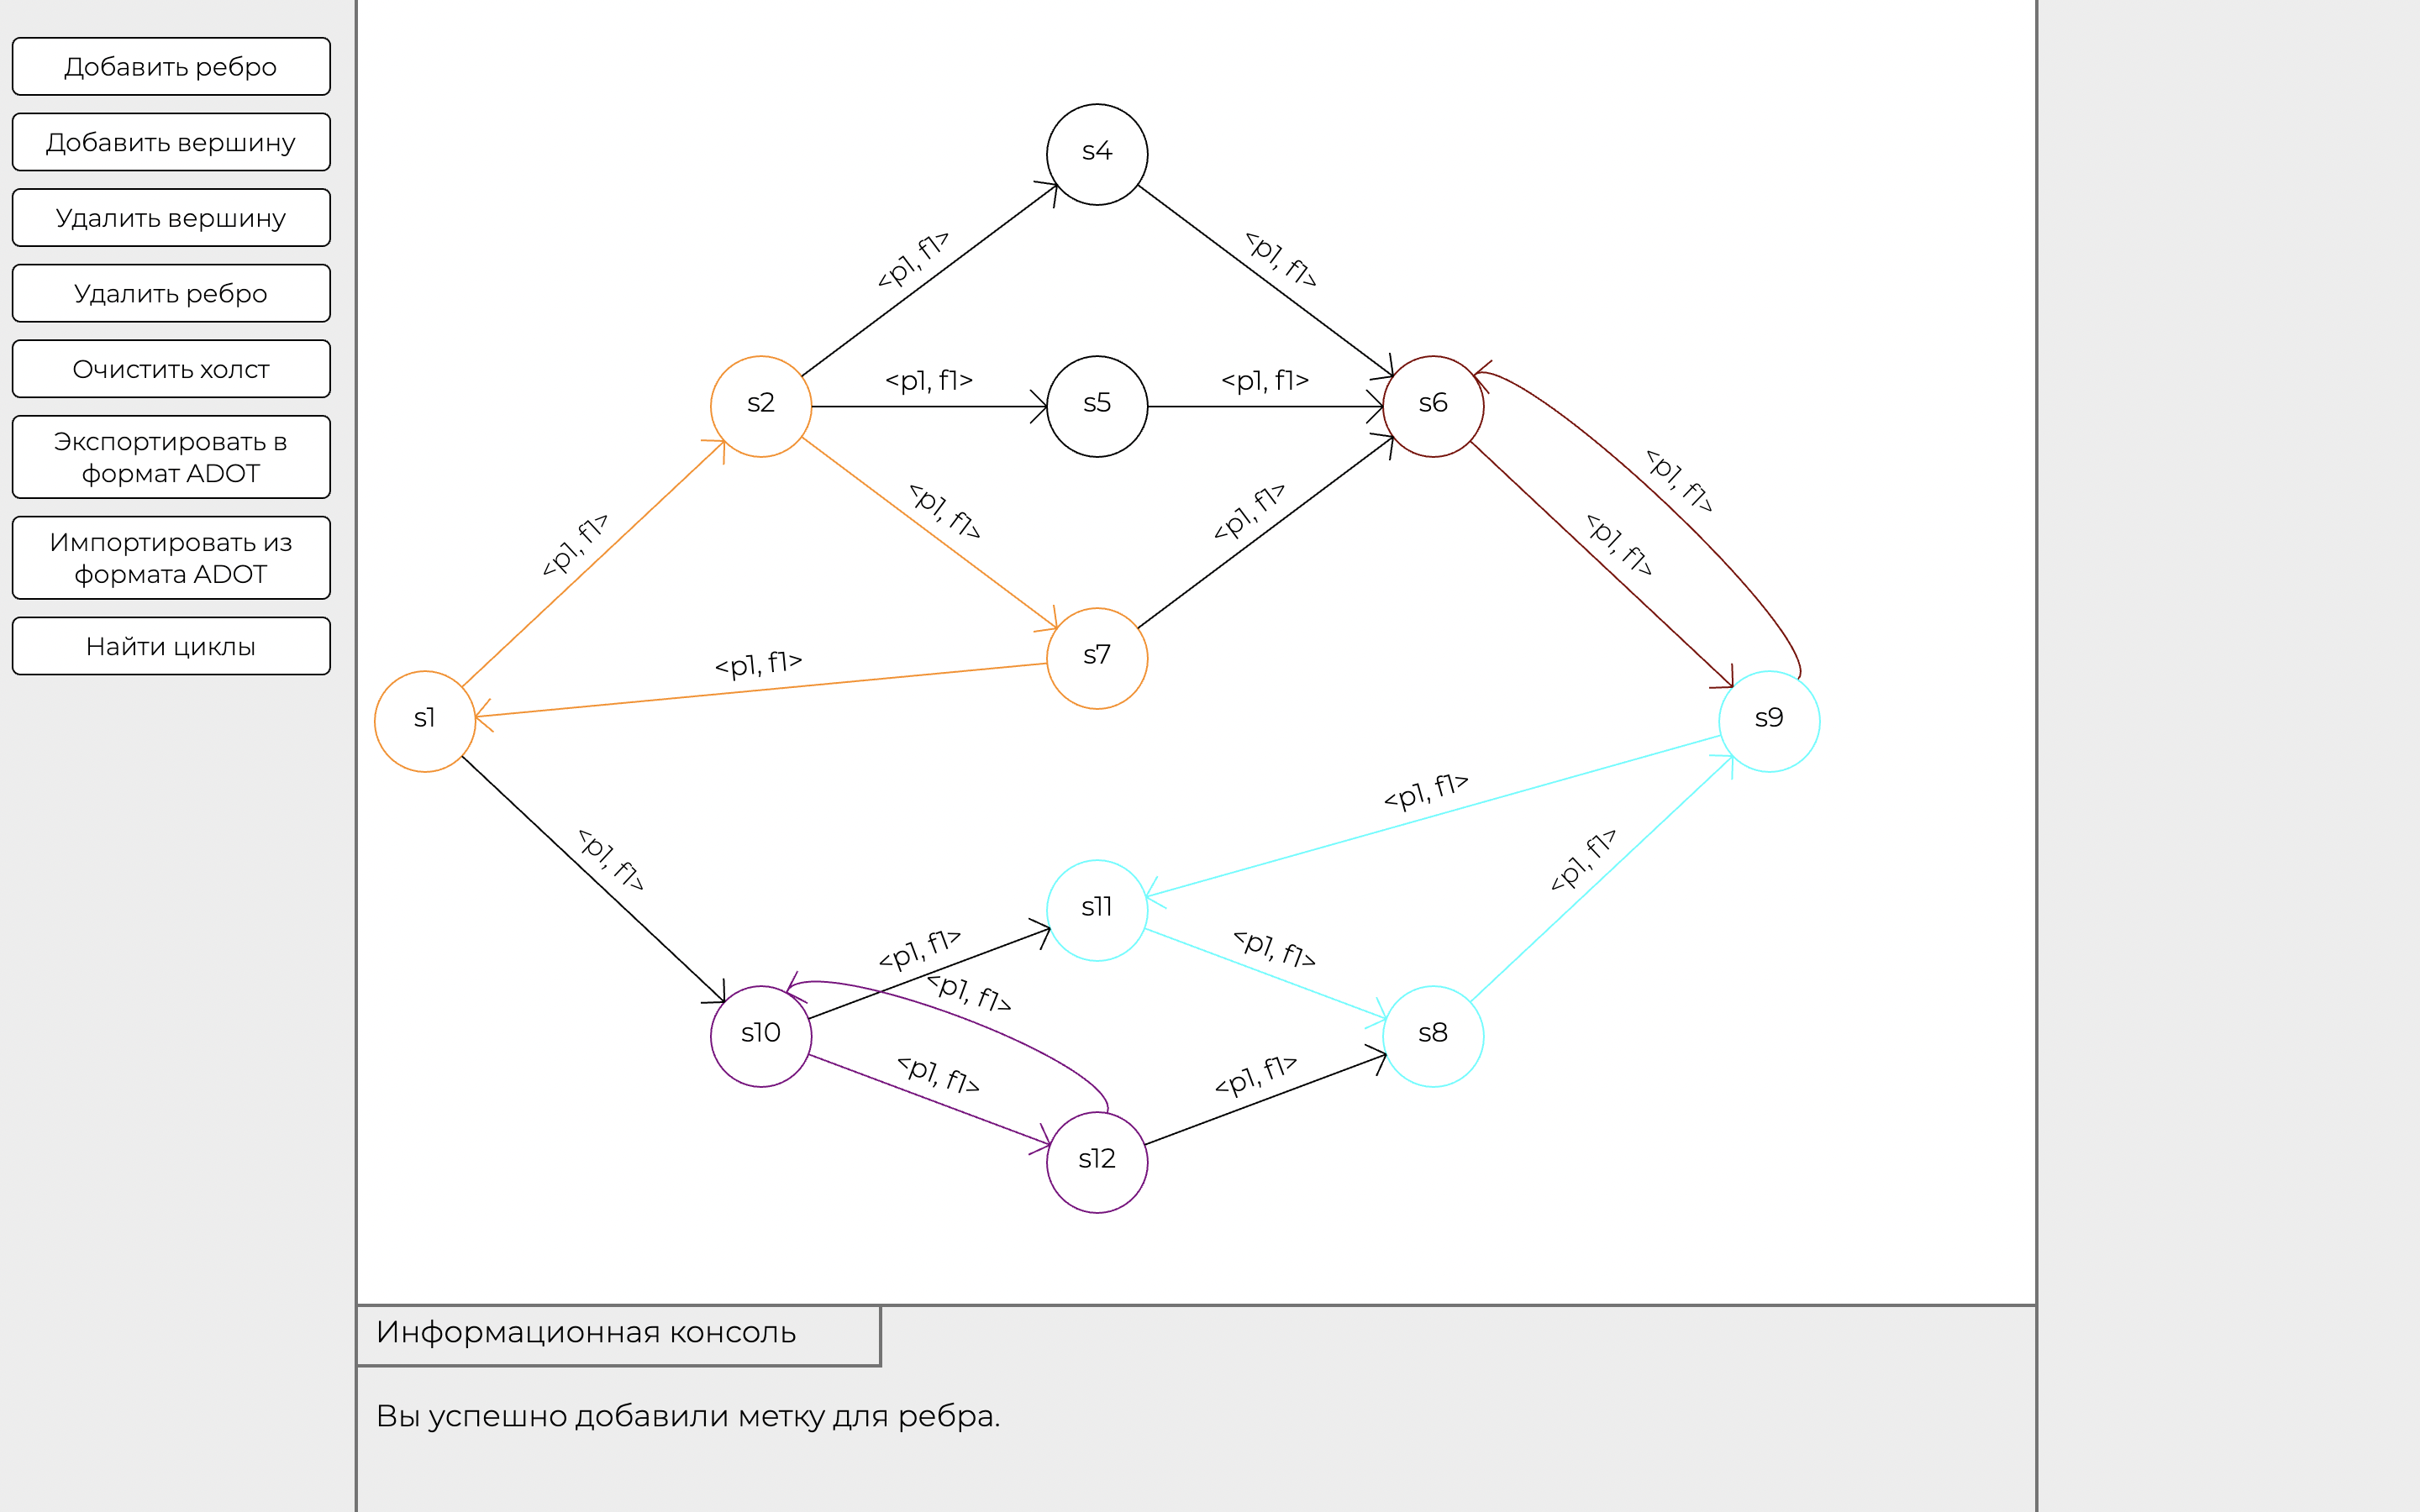
\includegraphics[width=0.75\linewidth]{images/example_many_cycles.png}}
\caption{Граф с множеством циклов}
\label{fig:example_many_cycles}
\end{figure}